\chapter{Design}
There have been several design ideas. 
\section{Map}
At the beginning we had a sidebar which could be visible or hidden. Later we found out that there is no need for a big menu, so we removed the sidebar and added a tiny top bar, with only the necessary options.\\
First mockup:\\
\begin{figure}[hbtp]
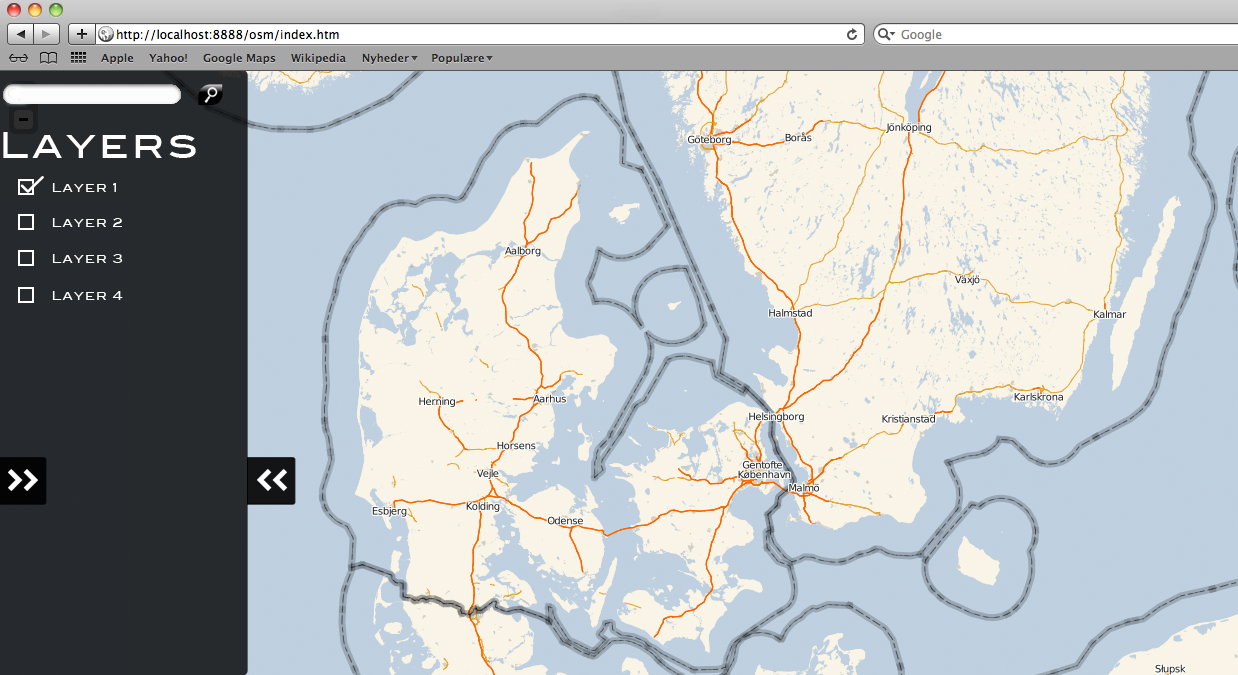
\includegraphics[scale=.5]{../figure/design_map_v1.png}
\caption{Map - version 1}
\end{figure}
We would like to have different layers on the map at the beginning, but this was unnecessary, so it was quickly removed.\\
Now we have created a cool design which is easy to get used to and all relevant informations can be accessed easily and without to much clicking.
There have also been added some gestures to control the radar easily.\\
The top bar has a date field to know which date the radar should get data from. This date will be transferred to the chart window.

\section{Chart}
At the beginning we had the same sidebar as on the map, but with other options. This was also replaced by a top bar like on the map.\\
First mockup:\\ 
\begin{figure}[hbtp]
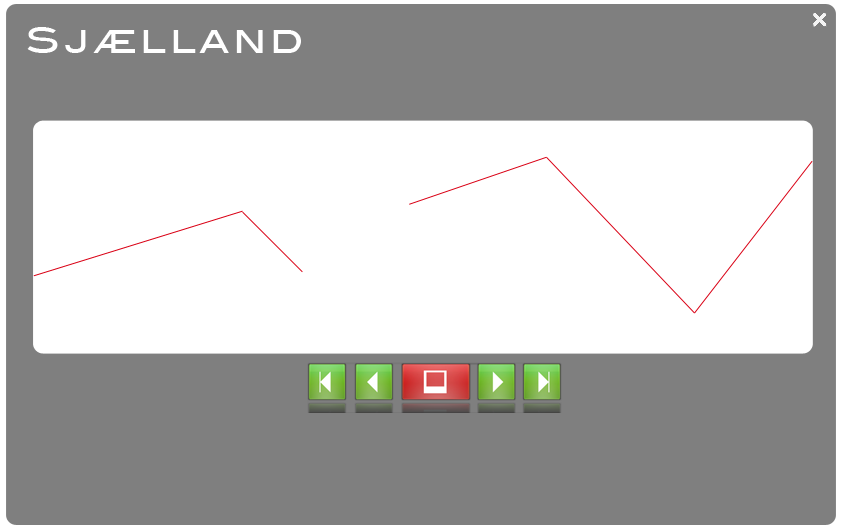
\includegraphics[scale=.5]{../figure/design_chart_v1.png} 
\caption{Chart pop up - version 1}
\end{figure}
This has, through the whole project, been determined to be a pop up on the map.
The control buttons were before 'fast backward', 'backward', 'today', 'forward' and 'fast forward', but 'today' was replaced with 'play'. The 'play' button moves the chart every second, so the user can view the chart animated.\\
The new design also have three different views '2-week', 'weekly' and 'daily view'. Control buttons adjust it self to the view the user has selected.